\documentclass[xetex,mathserif,serif]{beamer}
\usepackage{polyglossia}
\setdefaultlanguage[babelshorthands=true]{russian}
\usepackage{minted}
\usepackage{tabu}
\usepackage{moresize}

\useoutertheme{infolines}

\usepackage{fontspec}
\setmainfont{FreeSans}
\newfontfamily{\russianfonttt}{FreeSans}

\definecolor{links}{HTML}{2A1B81}
\hypersetup{colorlinks,linkcolor=,urlcolor=links}

\setbeamertemplate{blocks}[rounded][shadow=false]

\setbeamercolor*{block title alerted}{fg=red!50!black,bg=red!20}
\setbeamercolor*{block body alerted}{fg=black,bg=red!10}

\tabulinesep=1.2mm

\title{Работа с сетью}
\subtitle{Низкий уровень}
\author[Юрий Литвинов]{Юрий Литвинов\\\small{\textcolor{gray}{yurii.litvinov@gmail.com}}}
\date{04.10.2019г}

\newcommand{\attribution}[1] {
\vspace{-5mm}\begin{flushright}\begin{scriptsize}\textcolor{gray}{\textcopyright\, #1}\end{scriptsize}\end{flushright}
}

\begin{document}

	\frame{\titlepage}

	\section{Архитектура сети}

	\begin{frame}
		\frametitle{Архитектура глобальной сети}
		\begin{center}
			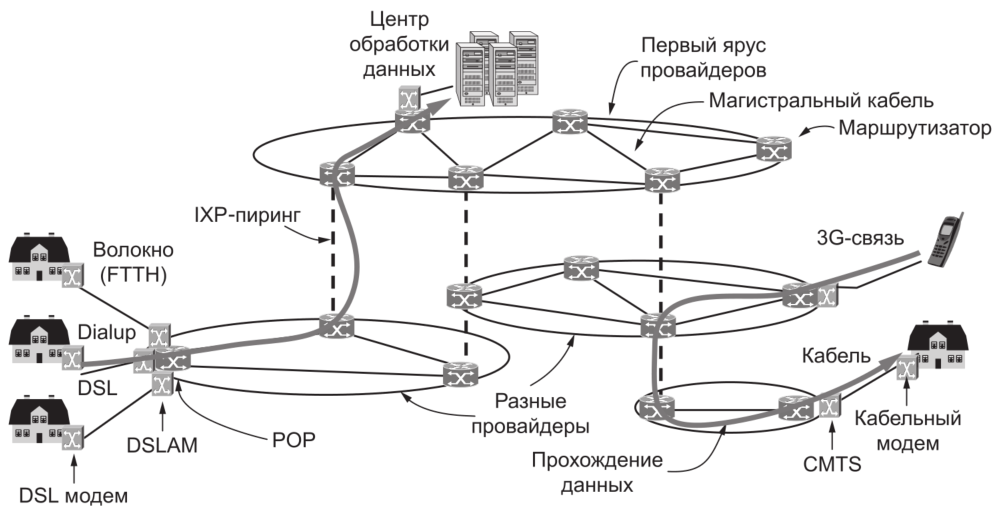
\includegraphics[width=0.9\textwidth]{internetArchitecture.png}
			\attribution{Э. Таненбаум}
		\end{center}
	\end{frame}

	\begin{frame}
		\frametitle{Уровневая архитектура}
		\framesubtitle{Модель OSI}
		\begin{center}
			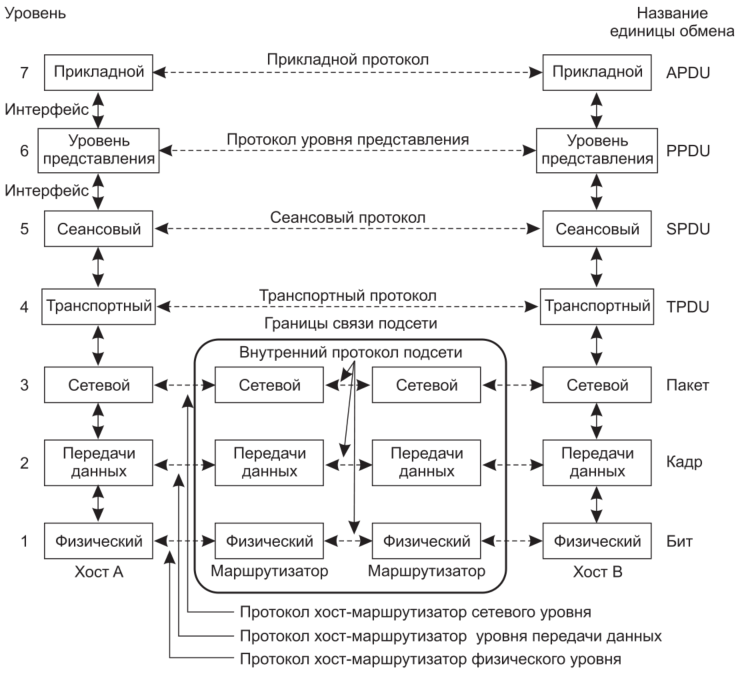
\includegraphics[width=0.6\textwidth]{osiStack.png}
			\attribution{Э. Таненбаум}
		\end{center}
	\end{frame}

	\begin{frame}
		\frametitle{Модель TCP/IP}
		\begin{center}
			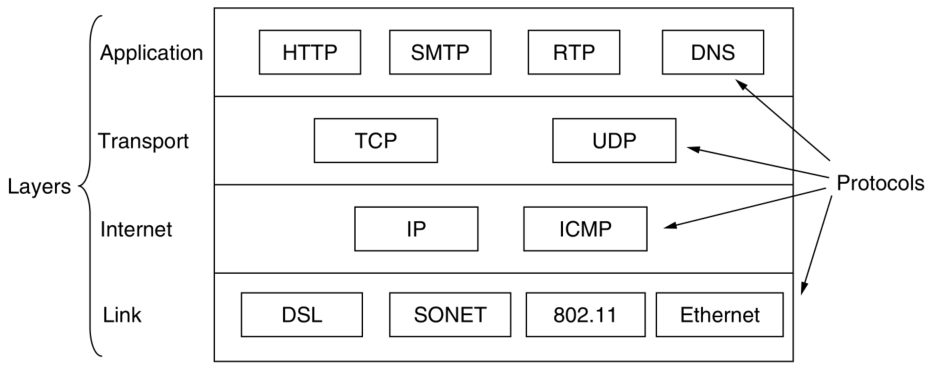
\includegraphics[width=0.9\textwidth]{tcpIpStack.png}
			\attribution{Э. Таненбаум}
		\end{center}
	\end{frame}

	\begin{frame}
		\frametitle{Физический уровень}
		\begin{itemize}
			\item Физические параметры канала (электрические, электромагнитные, ...)
			\item Ethernet (витая пара), USB, xDSL, Bluetooth, IEEE 802.11 (WiFi), оптические сети, спутниковая связь, мобильные сети (GSM, EDGE, LTE) и т.д.
			\begin{itemize}
				\item RFC 1149 ``IP over Avian Carriers'' (\url{https://tools.ietf.org/html/rfc1149})
			\end{itemize}
			\item Отвечает только за передачу сигнала в рамках среды распространения между двумя точками
			\item Вопросы кодирования битов уровнями сигнала, синхронизации, помехоустойчивости, мультиплексирования
			\item Передаёт биты или блоки битов
		\end{itemize}
	\end{frame}

	\begin{frame}
		\frametitle{Канальный уровень}
		\begin{itemize}
			\item Общение напрямую соединённых устройств сети
			\item PPP (Point to Point Protocol)
			\item Понятия MAC и LLC
			\begin{itemize}
				\item MAC-адрес: D8-FB-5E-E5-55-67
			\end{itemize}
			\item Вопросы коррекции ошибок физического уровня (коды Хэмминга, Рида-Соломона, свёрточные коды и прочая алгебра с теорией чисел), повтора передачи пропавших данных, управления скоростью передачи
			\item Передаёт фрэймы (или кадры)
		\end{itemize}
	\end{frame}

	\begin{frame}
		\frametitle{Сетевой уровень}
		\begin{itemize}
			\item Сеть из нескольких устройств
			\item Вопросы поиска оптимального маршрута внутри сети (роутинга), передачи по принципиально разным сетям (например, один пакет по оптоволокну, второй --- через спутник)
			\item IP (Internet Protocol)
			\item Понятие IP-адреса (IPv4, IPv6)
			\item Передаёт пакеты
		\end{itemize}
	\end{frame}

	\begin{frame}
		\frametitle{Транспортный уровень}
		\begin{itemize}
			\item Соединение двух устройств через сеть
			\item Вопросы надёжности доставки, разделения-сборки сообщения, правильного порядка сообщений, подтверждения и повторной отправки
			\item Протоколы TCP (Transmission Control Protocol), UDP (User Datagram Protocol)
			\begin{itemize}
				\item TCP --- протокол, гарантирующий доставку данных в правильном порядке, без потерь и порчи, если это вообще возможно
				\begin{itemize}
					\item Передача файлов, текстовых данных (включая веб-страницы), веб-сервисы
				\end{itemize}
				\item UDP --- протокол, позволяющий отправлять ``датаграммы'' без гарантий их доставки или доставки в правильном порядке, но в разы быстрее TCP
				\begin{itemize}
					\item Стриминг фильмов, музыки, компьютерные игры
				\end{itemize}
			\end{itemize}
		\end{itemize}
	\end{frame}

	\begin{frame}
		\frametitle{Сеансовый уровень}
		\begin{itemize}
			\item Установление, поддержание и закрытие соединения
			\item Протокол TCP
		\end{itemize}
	\end{frame}

	\begin{frame}
		\frametitle{Уровень представления}
		\begin{itemize}
			\item Кодировка и представление передаваемых данных
			\begin{itemize}
				\item Шифрование
				\item Сериализация/десериализация
			\end{itemize}
		\end{itemize}
	\end{frame}

	\begin{frame}
		\frametitle{Прикладной уровень}
		\begin{itemize}
			\item Общение конкретных приложений
			\item Протоколы HTTP, FTP, SMTP и т.д.
			\item Протоколы поверх HTTP: REST, SOAP и т.д.
		\end{itemize}
	\end{frame}

	\section{Технические детали}

	\begin{frame}
		\frametitle{IP-адреса}
		\begin{itemize}
			\item IPv4: 192.168.0.1 (4 байта)
			\begin{itemize}
				\item Уникален в рамках подсети (не глобально уникальный)
				\item 192.168.x.x, 172.16-31.x.x, 10.x.x.x --- адреса, зарезервированные для локальных подсетей
				\item 127.0.0.1 (точнее, 127.x.x.x) --- loopback (локальный адрес самого компа), часто используется для отладки
				\item Маска подсети --- битовая маска, определяющая кусок IP-адреса
			\end{itemize}
			\item IPv6: fe80::488f:1f6:9030:46c7\%10 (16 байт)
		\end{itemize}
	\end{frame}

	\begin{frame}
		\frametitle{Формат пакета IPv4}
		\begin{center}
			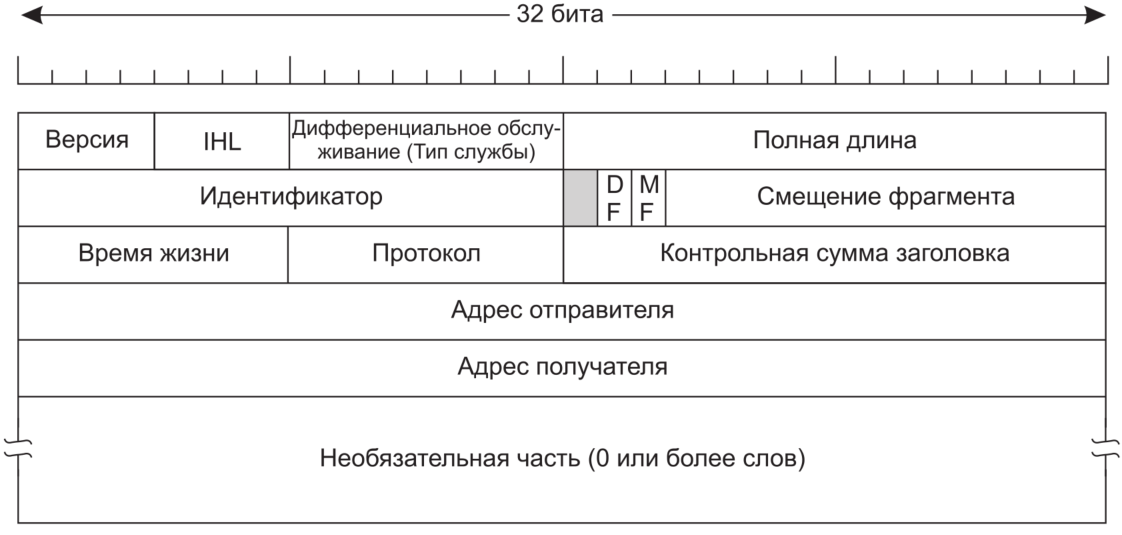
\includegraphics[width=0.9\textwidth]{ipv4.png}
			\attribution{Э. Таненбаум}
		\end{center}
	\end{frame}

	\begin{frame}
		\frametitle{DNS, NAT}
		\begin{itemize}
			\item DNS --- сопоставление непонятным IP-адресам читаемых доменных имён
			\begin{itemize}
				\item Более-менее глобальный сервис
				\item DNS-запрос по доменному имени (google.com) возвращает IP-адрес (64.233.164.113), только после этого возможен ``настоящий'' запрос
				\item Есть локальные DNS-сервера, есть общеизвестные (например, 8.8.8.8, Google Public DNS)
				\item localhost --- всегда (более-менее) раскрывается в 127.0.0.1
			\end{itemize}
			\item NAT --- Network Address Translation, механизм, позволяющий компьютерам с локальными IP получать ответы из Интернет (только если они инициировали запросы)
			\item Ports forwarding --- механизм, позволяющий компьютерам за NAT принимать входящие запросы
			\item Прокси --- программа, которая пересылает запросы (и может делать с ними что-нибудь)
		\end{itemize}
	\end{frame}

	\begin{frame}
		\frametitle{Порты и сокеты}
		\framesubtitle{Понятия транспортного/сеансового уровня}
		\begin{itemize}
			\item Порт --- число от 1 до 65535
			\item Привязан к сетевому интерфейсу
			\item Ресурс, управляемый ОС
			\item Типичные порты
			\begin{itemize}
				\item 22 --- SSH
				\item 25 --- SMTP
				\item 80 --- HTTP
				\item 443 --- HTTPS
				\item 666 --- Doom
				\item Первые 1024 порта зарезервированы
			\end{itemize}
			\item Ненужные порты обычно закрыты на уровне ОС (файерволл), чтобы было труднее взломать компьютер --- поэтому ваше первое сетевое приложение, скорее всего, не заработает
			\item Сокет --- программный интерфейс к порту
			\item Сетевой стек --- важная часть операционной системы, сокеты --- способ для прикладного программиста с ним работать
		\end{itemize}
	\end{frame}

	\begin{frame}
		\frametitle{Как работает NAT}
		\framesubtitle{Или ещё одна причина, почему ваше первое сетевое приложение не заработает}
		\begin{center}
			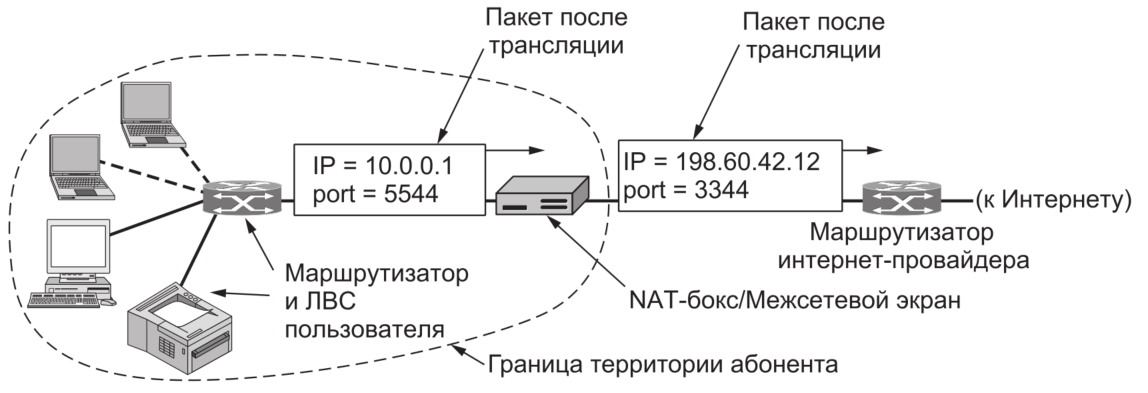
\includegraphics[width=0.9\textwidth]{nat.png}
			\attribution{Э. Таненбаум}
		\end{center}
	\end{frame}

	\begin{frame}
		\frametitle{Полезные консольные команды}
		\begin{itemize}
			\item ping --- проверка соединения с указанным IP или доменным именем, показывает время отклика узла
			\begin{itemize}
				\item Удалённый компьютер имеет право не отвечать
			\end{itemize}
			\item tracert (traceroute) --- показывает все узлы, через которые шёл запрос со временами их отклика (если они хотят откликнуться)
			\begin{itemize}
				\item Хороший способ диагностировать проблемы с интернетом
			\end{itemize}
			\item ipconfig под Windows, ifconfig под Linux --- узнать всё про локальный сетевой интерфейс (IP-адреса, MAC-адреса, используемые DNS и т.д.)
			\begin{itemize}
				\item Наиболее полезен ipconfig /all
			\end{itemize}
		\end{itemize}
	\end{frame}

	\begin{frame}[fragile]
		\frametitle{Полезные консольные команды (2)}
		\begin{itemize}
			\item netcat, nc --- позволяет опросить указанный порт или наоборот, прикинуться сервером, работающим по данному порту, очень полезна при отладке сетевых приложений
			\begin{itemize}
				\item Под Windows не входит в стандартную поставку, надо ставить отдельно
			\end{itemize}
			\item telnet --- открывает TCP-соединение с заданным хостом на заданный порт
			\begin{itemize}
				\item Пример:
				\begin{scriptsize}
					\begin{minted}{text}
telnet smtp.gmail.com 25
220 smtp.gmail.com ESMTP m71-v6sm2246896lje.84 - gsmtp
HELP
214 2.0.0  https://www.google.com/search?btnI&q=RFC+5321 m71-v6sm2246896lje.84 
    - gsmtp
					\end{minted}
				\end{scriptsize}
				\item Выйти --- Ctrl + `]', quit
				\item Под Windows не входит в стандартную поставку, надо ставить отдельно
			\end{itemize}
		\end{itemize}
	\end{frame}

	\section{Работа с сетью в .NET}

	\begin{frame}
		\frametitle{Работа с сетью в .NET}
		\begin{itemize}
			\item Пространство имён System.Net
			\item Классы TcpListener, TcpClient, UdpClient --- управляют стеком протоколов, предоставляют сокеты или потоки байтов
			\item Класс Socket --- абстракция сетевого соединения (сокета)
			\item Чаще всего в реальной жизни обработка запросов на сервере асинхронна --- каждый клиент обслуживается своей задачей в пуле потоков
			\item Dns --- класс, отвечающий за работу с DNS-службой
			\item IPEndPoint --- абстракция адреса (IP-адрес + порт)
		\end{itemize}
	\end{frame}

	\begin{frame}[fragile]
		\frametitle{Минимальный пример, сервер}
		\begin{footnotesize}
			\begin{minted}{csharp}
static void Main(string[] args)
{
    const int port = 8888;
    var listener = new TcpListener(IPAddress.Any, port);
    listener.Start();
    Console.WriteLine($"Listening on port {port}...");
    using (var socket = listener.AcceptSocket())
    {
        var stream = new NetworkStream(socket);
        var streamReader = new StreamReader(stream);
        var data = streamReader.ReadToEnd();
        Console.WriteLine($"Received: {data}");
    }
    listener.Stop();
}
			\end{minted}
		\end{footnotesize}
	\end{frame}

	\begin{frame}[fragile]
		\frametitle{Минимальный пример, клиент}
		\begin{footnotesize}
			\begin{minted}{csharp}
static void Main(string[] args)
{
    const int port = 8888;
    using (var client = new TcpClient("localhost", port))
    {
        Console.WriteLine($"Sending to port {port}...");
        var stream = client.GetStream();
        var writer = new StreamWriter(stream);
        writer.Write("Hello, world!");
        writer.Flush();
    }
}
			\end{minted}
		\end{footnotesize}
	\end{frame}

	\begin{frame}[fragile]
		\frametitle{Канал работает в обе стороны}
		\framesubtitle{Сервер}
		\begin{scriptsize}
			\begin{minted}{csharp}
static void Main(string[] args)
{
    const int port = 8888;
    var listener = new TcpListener(IPAddress.Any, port);
    listener.Start();
    Console.WriteLine($"Listening on port {port}...");
    using (var socket = listener.AcceptSocket())
    {
        var stream = new NetworkStream(socket);
        var reader = new StreamReader(stream);
        var data = reader.ReadLine();
        Console.WriteLine($"Received: {data}");

        Console.WriteLine($"Sending \"Hi!\"");
        var writer = new StreamWriter(stream);
        writer.Write("Hi!");
        writer.Flush();
    }
    listener.Stop();
}
			\end{minted}
		\end{scriptsize}
	\end{frame}

	\begin{frame}[fragile]
		\frametitle{Канал работает в обе стороны}
		\framesubtitle{Клиент}
		\begin{footnotesize}
			\begin{minted}{csharp}
static void Main(string[] args)
{
    const int port = 8888;
    using (var client = new TcpClient("localhost", port))
    {
        Console.WriteLine($"Sending \"Hello!\" to port {port}...");
        var stream = client.GetStream();
        var writer = new StreamWriter(stream);
        writer.WriteLine("Hello!");
        writer.Flush();

        var reader = new StreamReader(stream);
        var data = reader.ReadToEnd();
        Console.WriteLine($"Received: {data}");
    }
}
			\end{minted}
		\end{footnotesize}
	\end{frame}

	\begin{frame}[fragile]
		\frametitle{Немного асинхронности}
		\framesubtitle{Сервер}
		\begin{scriptsize}
			\begin{minted}{csharp}
static async Task Main(string[] args)
{
    const int port = 8888;
    var listener = new TcpListener(IPAddress.Any, port);
    listener.Start();
    Console.WriteLine($"Listening on port {port}...");
    using (var socket = await listener.AcceptSocketAsync())
    {
        var stream = new NetworkStream(socket);
        var reader = new StreamReader(stream);
        var data = await reader.ReadLineAsync();
        Console.WriteLine($"Received: {data}");

        Console.WriteLine($"Sending \"Hi!\"");
        var writer = new StreamWriter(stream);
        writer.AutoFlush = true;
        await writer.WriteAsync("Hi!");
    }
    listener.Stop();
}
			\end{minted}
		\end{scriptsize}
	\end{frame}

	\begin{frame}[fragile]
		\frametitle{Или, более типично}
		\framesubtitle{Сервер}
		\begin{scriptsize}
			\begin{minted}{csharp}
static async Task Main(string[] args) {
    const int port = 8888;
    var listener = new TcpListener(IPAddress.Any, port);
    listener.Start();
    Console.WriteLine($"Listening on port {port}...");
    while (true) {
        var socket = await listener.AcceptSocketAsync();
        Task.Run(async () => {
            var stream = new NetworkStream(socket);
            var reader = new StreamReader(stream);
            var data = await reader.ReadLineAsync();
            Console.WriteLine($"Received: {data}");

            Console.WriteLine($"Sending \"Hi!\"");
            var writer = new StreamWriter(stream);
            await writer.WriteAsync("Hi!");
            await writer.FlushAsync();

            socket.Close();
        });
    }
}
			\end{minted}
		\end{scriptsize}
	\end{frame}

	\begin{frame}[fragile]
		\frametitle{Теперь можно писать и читать одновременно}
		\framesubtitle{Полнодуплексное соединение, на примере сервера}
		\begin{scriptsize}
			\begin{minted}{csharp}
private static async Task Main(string[] args) {
    ...
    while (true) {
        var client = await listener.AcceptTcpClientAsync();
        Writer(client.GetStream());
        Reader(client.GetStream());
    }
}

private static void Writer(NetworkStream stream) {
    Task.Run(async () => {
        ...
    });
}

private static void Reader(NetworkStream stream) {
    Task.Run(async () => {
        ...
    });
}
			\end{minted}
		\end{scriptsize}
	\end{frame}

	\begin{frame}[fragile]
		\frametitle{Например}
		\begin{footnotesize}
			\begin{minted}{csharp}
private static void Writer(NetworkStream stream)
{
    Task.Run(async () =>
    {
        var writer = new StreamWriter(stream) { AutoFlush = true };
        while (true)
        {
            Console.WriteLine(">");
            var data = Console.ReadLine();
            await writer.WriteAsync(data + "\n");
        }
    });
}
			\end{minted}
		\end{footnotesize}
	\end{frame}

	\begin{frame}[fragile]
		\frametitle{UdpClient}
		\framesubtitle{Сервер}
		\begin{footnotesize}
			\begin{minted}{csharp}
static async Task Main(string[] args)
{
    const int port = 8888;
    var udpClient = new UdpClient(port);
    Console.WriteLine($"Listening on port {port}...");
    var received = await udpClient.ReceiveAsync();
    var data = Encoding.UTF8.GetString(received.Buffer);
    Console.WriteLine($"Received: {data}");
}
			\end{minted}
		\end{footnotesize}
	\end{frame}

	\begin{frame}[fragile]
		\frametitle{UdpClient}
		\framesubtitle{Клиент}
		\begin{footnotesize}
			\begin{minted}{csharp}
static async Task Main(string[] args)
{
    const int port = 8888;
    var udpClient = new UdpClient();

    Console.WriteLine($"Sending \"Hello!\" to port {port}...");
    var data = Encoding.UTF8.GetBytes("Hello!");
    await udpClient.SendAsync(data, data.Length, "localhost", port);
}
			\end{minted}
		\end{footnotesize}
		Не следует посылать UDP-датаграммы более 508 байт размером
	\end{frame}

\end{document}
